\documentclass[../Main.tex]{subfiles}

\begin{document}
\section{Motion in One Dimension}
Often, we can reduce problems to motion in one dimension. In one dimension, Newton's Second Law is:
\begin{equation}
    m\ddot{x} = F_x
    \label{eqnNewtonSecondOneDim}
\end{equation}
If $F_x$ is velocity independent, then it can always be written as a gradient of a potential:
\begin{equation}
    V(x) = -\int_{x_0}^{x} F_x(u) du
    \label{eqnPotentialOneDim}
\end{equation}
\subsection{Finding an Integral}
Then we can conserve an energy $E = \frac{1}{2} m \dot{x}^2 + V(x)$. Solving this as a first-order differential equation:
\begin{equation}
    t - t_0 = \pm \int_{x_0}^x \frac{du}{\sqrt{\frac{2}{m}\left(E - V(u)\right)}}
    \label{eqnTimeGivenEnergy}
\end{equation}
Such a formula is only easy to derive for 1 dimension. In more dimensions something like this may not even be possible to find. Even still, this integral is rarely able to be solved, especially for more complex systems.
\subsection{Potential and Stationary Points}
We can try to understand 1-dimensional motion without computing the integral in equation~\ref{eqnTimeGivenEnergy}. Considering the energy:
\begin{align*}
    E &= \frac{1}{2} m \dot{x}^2 + V(x) \\
    &\geq V(x) \text{ since the kinetic energy is} \geq 0
\end{align*}
So this restricts the places that a particle can be: for a particle of measured energy $E$, it cannot exist in such coordinates $x$ such that $V(x) > E$. Also, for coordinates $x$ such that $V(x) = E$, then $\dot{x}$ must equal 0 there. Such points are called turning points, because the particle must change direction at these points. \par
\begin{figure}[ht]
    \centering
        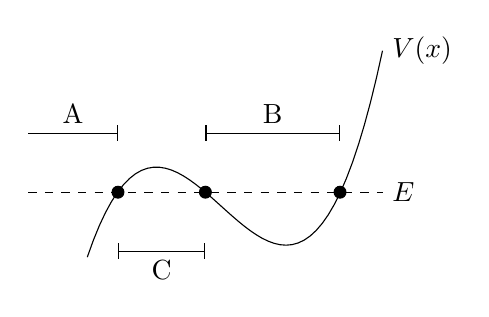
\begin{tikzpicture}[scale=1.5]
            \draw[domain=-0.5:2, samples=50] plot (\x, {\x * \x * \x -1.9 * \x * \x + 0.3 * \x + 1.2}) node[right] {$V(x)$};
            \draw[dashed] (-1, 1) -- (2, 1) node[right] {$E$};
            \draw[-Bar] (-1, 1.5) -- (-0.24, 1.5) node[pos=0.5, anchor=south] {A};
            \draw[Bar-Bar] (-0.24, 0.5) -- (0.5, 0.5) node[pos=0.5, anchor=north] {C};
            \draw[Bar-Bar] (0.5, 1.5) -- (1.64, 1.5) node[pos=0.5, anchor=south] {B};
            \foreach \x in {-0.24, 0.5, 1.64}
                \draw[fill] (\x, 1) circle[radius=0.5mm];
        \end{tikzpicture}
    \caption{Regions for a given potential and energy of a particle}
    \label{figPotentialPlot}
\end{figure}
In figure~\ref{figPotentialPlot}, we have two regions. In region B, the particle motion is of bouncing back and forth between the two turning points. In region A, the particle can reach the turning point, and then fly off to $-\infty$. The particle cannot exist in region C.\par
A special case occurs when $E = V(x)$ and furthermore $V'(x) = 0$. These are called equilibrium points. Here it is possible for the particle to lie stationary:
\begin{align*}
    V = E &\implies \dot{x} = 0 \\
    m\ddot{x} &= -V'(x) = 0
\end{align*}
And thus at an equilibrium point $\ddot{x} = \dot{x} = 0$.\par
Motion close to an equilibrium point is especially simple, depending only on the curvature of $V(x)$ around the stationary point. Let $x_0$ be the equilibrium point and $x$ be the position of a particle, where $x$ is close to $x_0$.
\begin{align}
    V(x) &= V(x_0) + (x - x_0)V'(x_0) + \frac{1}{2}(x - x_0)^2 V''(x_0) + O((x - x_0)^3) \nonumber \\
    &\approx V(x_0) + \frac{1}{2}(x - x_0)^2 V''(x_0) \label{eqnStationaryOneDimMotion}
\end{align}
In the case where $V''(x_0) > 0$, we have the potential for a harmonic oscillator:
\begin{equation*}
    m\ddot{x} = -V(x) \approx (x-x_0)V''(x)
\end{equation*}
And $x(t)$ gives small oscillations about $x_0$, with frequency $\omega = \sqrt{\frac{V''(x_0)}{m}}$.\par
In the case where $V''(x_0) < 0$, we have an unstable equilibrium point:
\begin{equation*}
    x = x_0 Ae^{\gamma t} + Be^{-\gamma t}
\end{equation*}
where $\gamma = \sqrt{-\frac{V''(x_0)}{m}}$. Solutions to $x(t)$, for $A \neq 0$, display exponential growth and are thus unstable. Solutions with $A = 0$ correspond to the ball having exactly enough energy to reach the equilibrium point and stop there.\par
In the case $V''(x_0) = 0$, higher-order terms are needed. If $V(x)$ is not twice-differentiable at $x_0$, special consideration is needed for the specific case.
\end{document}